\documentclass[12pt]{article}
\usepackage[utf8]{inputenc}
%\usepackage[portuguese]{babel}
\usepackage{amsmath,amsfonts,amssymb}
\usepackage{graphicx}
\usepackage{makeidx}
\usepackage{graphicx}
\usepackage{lmodern}
\usepackage{multicol}
\usepackage{booktabs}
\usepackage{fancyhdr}
\usepackage{hyperref}
\usepackage[usenames]{color}


\usepackage{Sweave}
\begin{document}
\Sconcordance{concordance:SVM.tex:SVM.Rnw:%
1 15 1 1 0 47 1 1 2 1 0 6 1 1 2 3 1 1 2 4 1 3 0 1 2 2 1 1 21 23 0 1 2 5 %
1 1 2 1 0 4 1 3 0 1 2 2 1 1 2 13 0 1 2 3 1 1 3 1 2 5 1 1 20 1 2 5 1 1 4 %
1 2 17 1}

\pagestyle{fancy}
\fancyhf{}
\renewcommand{\headrulewidth}{0.4pt}
\fancyfoot[C]{\thepage}
\renewcommand{\footrulewidth}{0.4pt}
\fancyfoot[C]{\thepage}
\title{\LARGE \bf
 Exercício 4 - SVM}
\author{ Rodrigo Machado Fonseca - 2017002253}
\thispagestyle{fancy}
\fancyhead[C]{Introdução ao Reconhecimento de Padrões - UFMG \\ Belo Horizonte - \today}
\maketitle
\thispagestyle{fancy}

%%%%%%%%%%%%%%%%%%%%%%%%%%%%%%%%%%%%%%%%%%%%%%%%%%%%%%%%%%%%%%%%%%%%%%%%%%%%%%%%%%%%%%%%%
\section{Introdução}

  \par Neste exercício vamos aplicar o classificador SVM na resolução de um problema de classificação. Para isso será utilizado o conjunto de dados espiral do pacote \textit{mlbench}. Deveremos treinar uma SVM para separar as duas classes de amostras, verificar o hiperplano de separação gerado e testar o classificador para um conjunto de teste.
  
\section{\textit{Support Vector Machine} - SVM}
  
  \par \textit{Support Vector Machine} (SVM) é um algoritmo de aprendizado de máquina supervisionado que pode ser usado para desafios de classificação ou regressão.
  
  \par No caso de classificação trata-se de um problema multi-objetivo que minimiza o erro e maximiza a margem. Esse algoritmo, resolve apenas problemas lineares, porém, com a incorporação das funções de kernel é possível mapear as amostras em um espaço de dimensões N que este torna-se linearmente separável. O problema resume as seguintes equações:
  \begin{center}
    Dados o parâmetro C e a matriz Z, encontre Multiplicadores de Lagrange $\alpha_i$ que minimiza a função 
  \end{center}
  
  \begin{equation}
  W(\alpha) = \sum_{i=1}^{N}\alpha_i -0.5*\sum_{i=1}^{N}\sum_{j=1}^{N}\alpha_i\alpha_jK(x_i,x_j,z).
  \end{equation}
  
  \begin{center}
   e que satisfaçam as seguintes restrições:
    \begin{itemize}
    \item $\sum_{i=1}^{N}\alpha_i= 0$
    \item $0\leq \alpha_i  \leq C$
    \end{itemize}
  \end{center} 

  \par A formulação de um SVM com margens flexíveis conforme descrita na equação anterior possui função de custo convexa e restrições lineares, o que garante a existência de um mínimo global. Para que o problema seja solucionado precisamos fornecer, a priori, um determinado K e C. A condição de atingir o mínimo global depende desses parâmetros. Para atingirmos o mínimo global é necessário buscar K's e C's, de forma discreta, com o intuito que um satisfaça essa condição. Ao fazermos a busca não há garantia que atingiremos o mínimo global. 


\section{Metodologia}
  \par A priori, carregou-se a base de dados \textit{mlbench.spirals}, e foram guardados os valores de x e de y. Em sequência, separou-se 70\% do conjunto de dados para teste e 30\% para treinamento.

\begin{Schunk}
\begin{Sinput}
> rm(list = ls())
> library(mlbench)
> library('RSNNS')
> library('kernlab')
> data <- mlbench.spirals(500, sd = 0.05)
> x <- cbind(as.matrix(data[["x"]]))
> y <- sign(as.matrix(as.numeric(data[["classes"]]))-1.5)
> set.seed(13)
> index <- sample(1:nrow(x), length(1:nrow(x)))
> x <- x[index,1:ncol(x)]
> y <- y[index,1]
> training_sample_number = round(nrow(x)*0.7)
> x_train <- x[1:training_sample_number,]
> y_train <- y[1:training_sample_number]
> x_test <- x[(training_sample_number+1):nrow(x), ]
> y_test <- y[(training_sample_number+1):nrow(x)]
\end{Sinput}
\end{Schunk}

  \par Em seguida, utilizou-se a função \textit{ksvm} para construir o classificador SVM. Vale ressaltar que foram escolhidos como parâmetros dessa função o kernel "C-bsvc" e os parâmetro "kpar" e "C" foram escolhidos de forma arbitrária.

\begin{Schunk}
\begin{Sinput}
> training_svm <- function(x_train, y_train, x_test, y_test, r, C_par){
+   best_accuracy <- 0
+   best_value <- 0
+   accuracy_list <- c()
+   for(i in 1:length(r)){
+     svm <- ksvm(x_train,y_train,type='C-bsvc',
+                 kernel='rbfdot',
+                 kpar=list(sigma=r[i]),
+                 C=C_par[i])
+     y_hat <- predict(svm, x_test)
+     accuracy <- 1 - (t(y_test - y_hat) %*% (y_test - y_hat))/length(y_test)
+     accuracy_list <- c(accuracy_list, accuracy)
+     if(accuracy > best_accuracy){
+       best_accuracy <- accuracy
+       svm_salve <- svm
+       best_value <- i
+     }
+   }
+   return(list(svm_salve, accuracy_list, best_value))
+ }
\end{Sinput}
\end{Schunk}

  \par Para a realização dos testes, foi utilizada a função \textit{predict} para obter os rótulos das amostras de teste. Em seguida, comparou-se os rótulos obtidos com os rótulos originais da amostra. Essa comparação foi feita por meio do cálculo da acurácia. Os resultados obtidos serão mostrados na seção seguinte. 

\section{Resultados}

  \par Os valores "kpar" e "C" utilizados para encontrar um mínimo global correspondem a "r" e "C\_par" no seguinte trecho de código:
\begin{Schunk}
\begin{Sinput}
> r <- c(0.1, 0.1, 0.1, 1.5, 1.5, 1.5, 0.2, 0.2, 0.2)
> C_par <- c(10, 100, 1000, 10, 100, 1000, 10, 100, 1000)
> results <- training_svm(x_train, y_train, x_test, y_test, r, C_par)
> svm <- results[[1]]
> accuray_list <- results[[2]]
\end{Sinput}
\end{Schunk}

  \par Para o treinamento obtivemos os seguintes valores de acurácia:

\begin{Schunk}
\begin{Soutput}
  accuray_list
1    0.4400000
2    0.6800000
3    0.9200000
4    1.0000000
5    1.0000000
6    1.0000000
7    0.6533333
8    0.9466667
9    0.9733333
\end{Soutput}
\end{Schunk}

  \par É possível ver o gráfico das amostras com o vetor suporte (Figura \ref{1}), o gráfico com a separação das classes (Figura \ref{2}) e a superfície de separação (Figura \ref{3}).
\begin{figure}[!h]
\centering
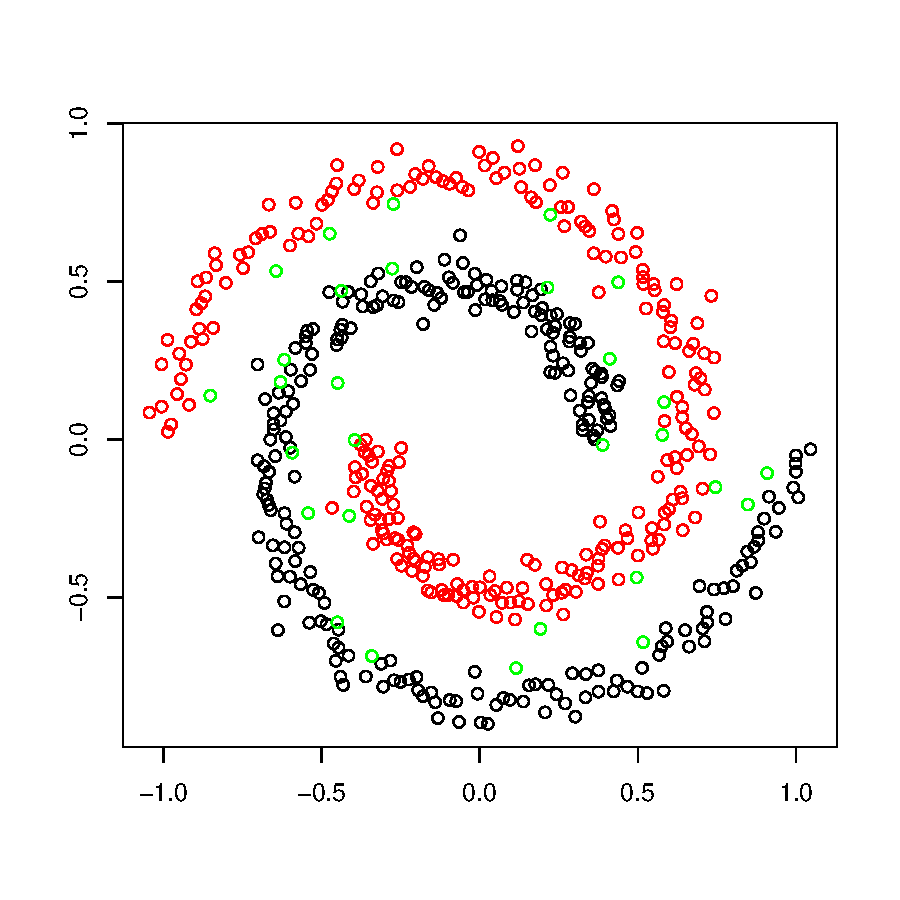
\includegraphics{SVM-005}
\caption{Amostras do cojunto de dados com vetores de suporte em verde.}
\label{1}
\end{figure}

\begin{figure}[!h]
\centering
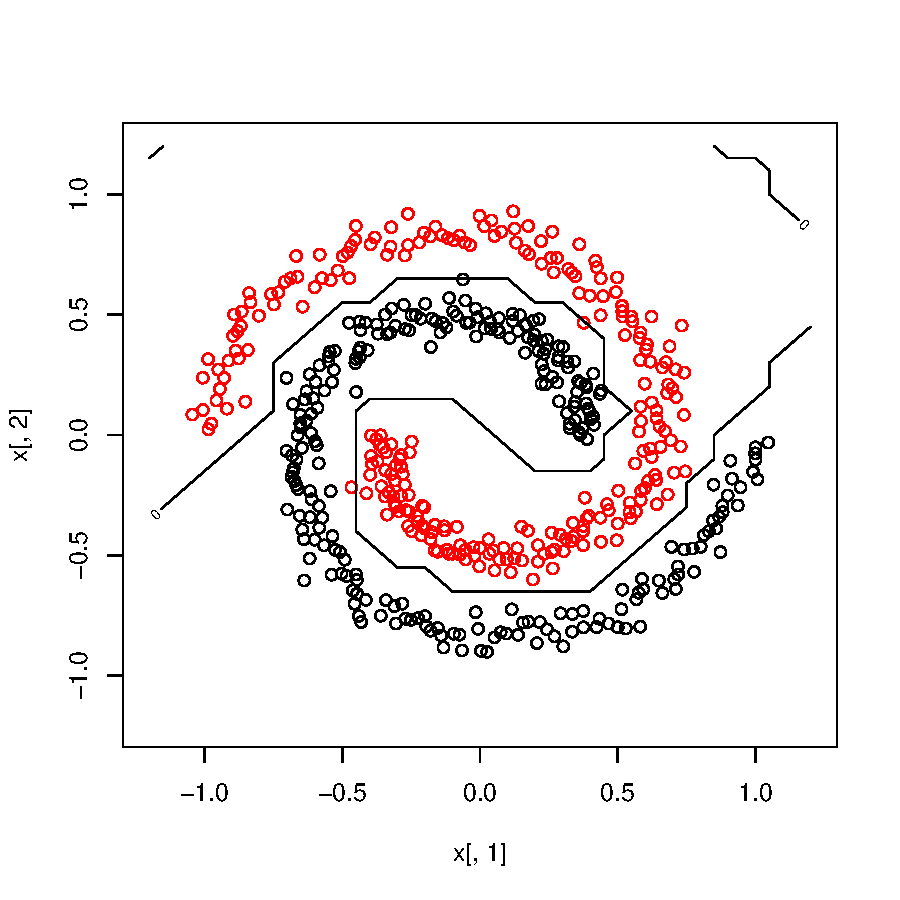
\includegraphics{SVM-006}
\caption{Hiperplano de separação das classes}
\label{2}
\end{figure}

\begin{figure}[!h]
\centering
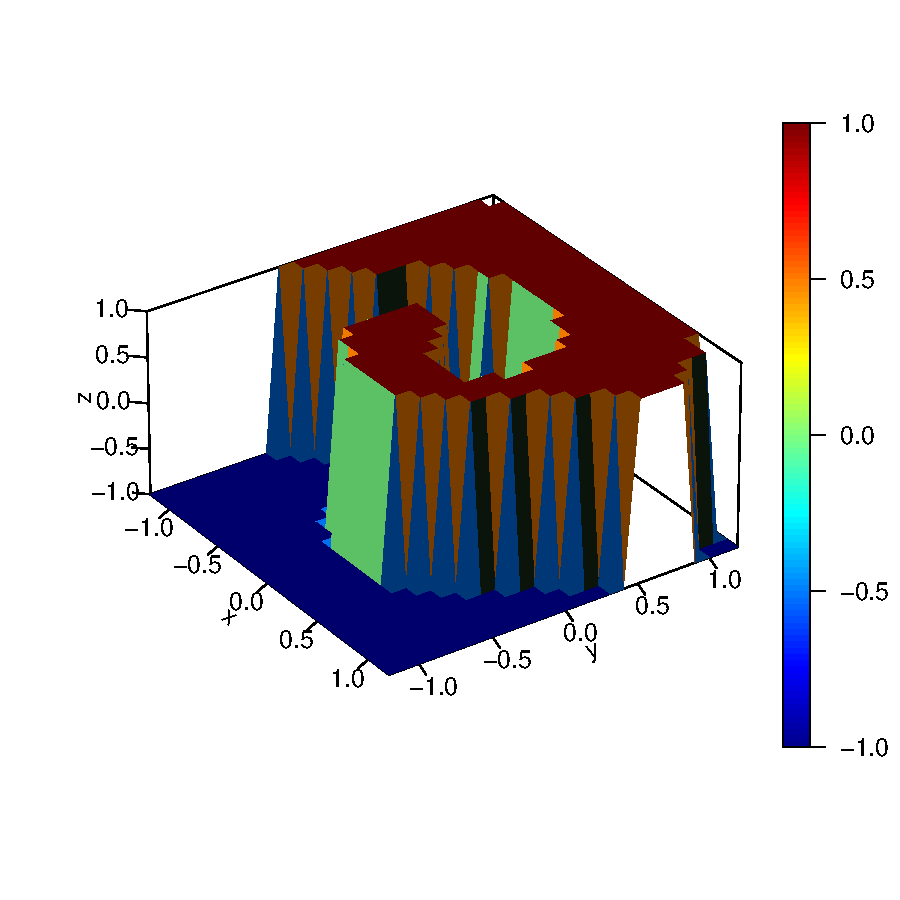
\includegraphics{SVM-007}
\caption{Superfície de separação das classes}
\label{3}
\end{figure}

\section{Discussão}

  \par Ao analisarmos a acurácia obtida, podemos ver que ao aumentar o valor de C, para um mesmo "kpar", a acurácia aumenta. Já o parâmetro "kpar" igual a 1.5 mostrou o melhor de todos, pois conseguiu valor máximo independente do valor de C.  
  \par Por meio da figura \ref{1}, foi possível observar os vetores de suporte selecionados, com o intuito de visualizar melhor o comportamento do algoritmo de SVM. É possível notar que a maioria dos vetores de suporte estão nos pontos de "curva" do hiperplano separador.
  \par Neste exercício não foi possível determinar uma maneira para começarmos o a busca pelo parâmetros "kpar" e "C". Logo, caso não obtivessemos um resultado satisfatório seria necessário aumentar o espaço de busca até melhorarmos o resultado. Fazer isso de forma cega pode ser muito custoso computacionalmente em alguns casos. Portanto, seria interessante de forma precisa limitarmos o espaço de busca.
  \par Além disso, foi possível observar que para um mesmo par "kpar" e "C" o algoritmo converge para respostas diferentes. Isso ocorre pelo fato de escolher o conjunto treino e teste de forma aleatória. Uma forma de minimizar isso seria escolher de forma balanceada as amostras, de modo que cada classe obtivesse o mesmo número de amostras.  
   \par Neste experimento foi possível analisar o comportamento do algoritmo SVM, além de que conseguimos construir e validar um classificador SVM.
%%%%%%%%%%%%%%%%%%%%%%%%%%%%%%%%%%%%%%%%%%%%%%%%%%%%%%%%%%%%%%%%%%%%%%%%%%%%%%%%%%%%%%%%%

%%%%%%%%%%%%%%%%%%%%%%%%%%%%%%%%%%%%%%%%%%%%%%%%%%%%%%%%%%%%%%%%%%%%%%%%%%%%%%%%%%%%%%%%%



\end{document}
